\begin{figure}[h]
    \centering
    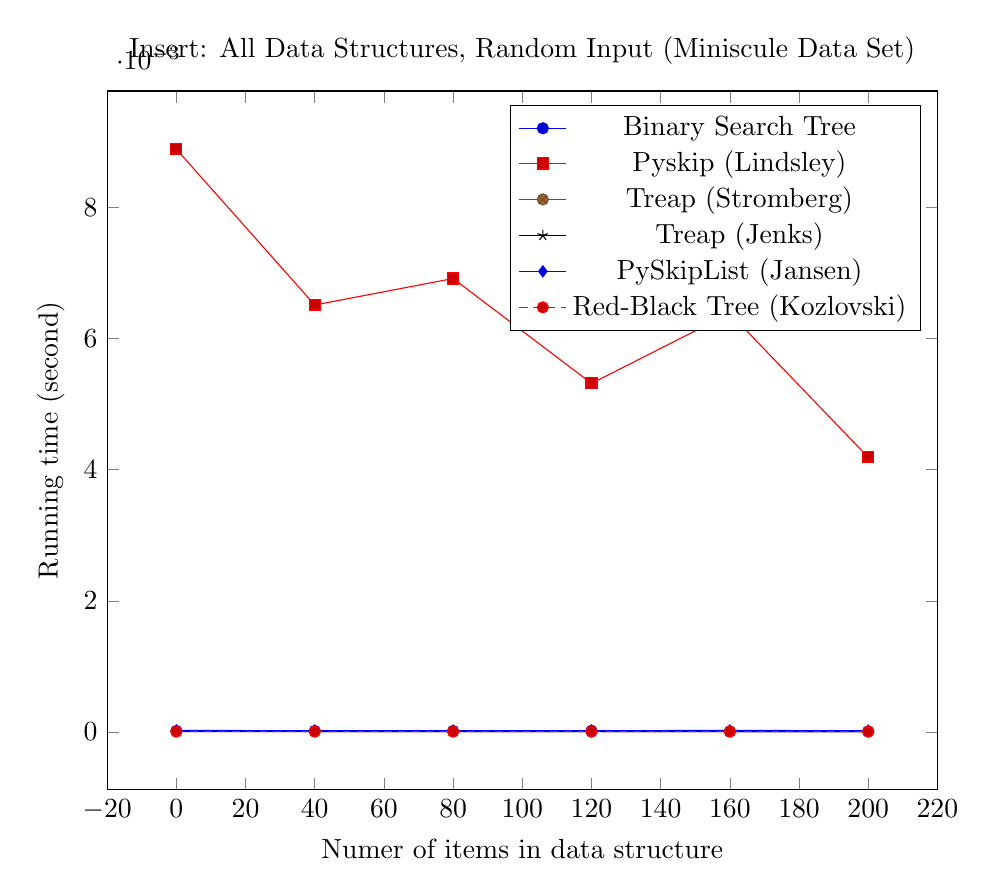
\begin{tikzpicture}
        \begin{axis}[
            xlabel={Numer of items in data structure},
            ylabel={Running time (second)},
            title={Insert: All Data Structures, Random Input (Miniscule Data Set)},
            width=\textwidth
        ]
		\addplot coordinates {
			(0, 1.4064888226306138e-05)
			(40, 1.3673360288546377e-05)
			(80, 1.319147974969681e-05)
			(120, 1.6142998049861745e-05)
			(160, 5.481391128858704e-06)
			(200, 5.391038527857717e-06)
		};
		\addplot coordinates {
			(0, 0.008893737811810621)
			(40, 0.006514964649544819)
			(80, 0.006919503361869683)
			(120, 0.0053185155067651205)
			(160, 0.0063875975996325884)
			(200, 0.0041900416374902605)
		};
		\addplot coordinates {
			(0, 7.5595009525031285e-06)
			(40, 5.330803460523726e-06)
			(80, 4.336924849202006e-06)
			(120, 4.397159916624815e-06)
			(160, 5.180215792144338e-06)
			(200, 5.2404508594783294e-06)
		};
		\addplot coordinates {
			(0, 2.710578030740152e-06)
			(40, 2.439520227692782e-06)
			(80, 2.2286974919794033e-06)
			(120, 2.3190500929359813e-06)
			(160, 2.1082273573114206e-06)
			(200, 2.5901078959833514e-06)
		};
		\addplot coordinates {
			(0, 1.981733715830103e-05)
			(40, 1.8401813075552553e-05)
			(80, 1.6926053925381267e-05)
			(120, 1.8582518277554526e-05)
			(160, 1.9606514422587652e-05)
			(200, 1.8522283210220537e-05)
		};
		\addplot coordinates {
			(0, 2.770813098074143e-06)
			(40, 2.9515183001649346e-06)
			(80, 3.162341035878313e-06)
			(120, 3.523751439971079e-06)
			(160, 3.523751439971079e-06)
			(200, 3.493633906348492e-06)
		};
        \legend{Binary Search Tree, Pyskip (Lindsley), Treap (Stromberg), Treap (Jenks), PySkipList (Jansen), Red-Black Tree (Kozlovski)}
        \end{axis}
    \end{tikzpicture}
    \caption{Average of 10 operations, benchmarked every 40, starting at 0.}
\end{figure}